\documentclass{article}
\usepackage{graphicx} % Requis pour insérer des images
\usepackage{fancyhdr} % Pour personnaliser les en-têtes/pieds de page
\usepackage[colorlinks=true, urlcolor=blue, linkcolor=red]{hyperref}
\usepackage[a4paper, margin=3cm]{geometry}
\usepackage{tabularx}
\usepackage{float}

\graphicspath{ {./tests_python/} {./rendu/}} 

\title{Daemon de Contrôle Distribué : Rapport de Projet}
\author{
    Fieux Telmo, Fort Alexandre, Lagier Hadrien, Maati Mohamed-Yâ-Sîn \\
    \textit{Université de Toulouse} \\
    Dirigé par : Poquet Millian
}
\date{Mai 2025}
\begin{document}

\pagestyle{fancy}
\fancyhf{} % Nettoie les en-têtes/pieds existants
\fancyhead[L]{Université de Toulouse: Rapport démon de contrôle} % Gauche
\fancyhead[R]{\thepage} % Numéro de page à droite

\maketitle
\newpage
\tableofcontents % génère le sommaire
\newpage

%----------------------------------------------------------------------------------------------
\section{Introduction}

\subsection{Présentation du projet}

L’expérimentation réelle est une méthode essentielle pour l’étude des systèmes et applications distribuées en informatique. Elle consiste à exécuter de manière contrôlée de vraies
applications distribuées sur des systèmes réels, permettant ainsi d’observer et d’analyser leur
comportement afin d’en extraire des connaissances.\\

Bien que de nombreux outils permettent de lancer des programmes à distance (\texttt{sshd}, peu offrent la
robustesse, la remontée d’erreurs efficace, et la faible interférence nécessaires pour des expériences scientifiques rigoureuses.

\subsection{Objectifs}

Ce projet vise à développer une application distribuée \textbf{légère}, \textbf{robuste} et \textbf{asynchrone} conçue pour \textbf{exécuter et contrôler des processus} à travers un réseau de machines. L'application sera \textbf{implémentée} en \textbf{Rust} et en \textbf{C}, avec des comparaisons de performances et de conception entre les deux langages afin de mieux répondre aux exigences du projet.\newline

Nous appelons cette application un \textit{Daemon de Contrôle}. Elle suit une \textbf{architecture basée sur des démons}, dans laquelle un processus de longue durée fonctionne sur chaque machine, offrant une interface de contrôle à distance. La communication entre les composants est assurée via le \textbf{protocole TCP}, et les commandes sont échangées à l'aide d'un mécanisme de \textbf{sérialisation inter-langages}.\\

Pour l'implémentation asynchrone en Rust, nous utilisons la bibliothèque \href{https://docs.rs/tokio/latest/tokio/}{Tokio}, qui fournit des outils puissants pour la concurrence et les entrées/sorties non bloquantes.


%----------------------------------------------------------------------------------------------
\section{État de l’art et veille technologique}

\subsection{Outils et technologies comparés}

\subsubsection{Sérialisation des données}


La sérialisation des données est essentielle pour la communication réseau. Elle transforme des structures complexes en une séquence d'octets, ce qui va nous permettre de transporter facilement différents types de données, ainsi que de faire communiquer des programmes de différents langages ensemble, une fonctionnalité qui nous sera utile lors des tests de régression et de performance.

Après une étude des différentes options qui s'offraient a nous, nous avons décidé d'utiliser Flatbuffers, une bibliothèque de sérialisation \textit{cross-platform} qui supportent des langages tels que C, Python et Rust. Cette bibliothèque ayant été initialement créée pour des applications à fort enjeu de performance, elle correspond parfaitement a notre projet.

\subsubsection{Technologies réseau}

\begin{table}[H]
    \centering
    \caption{Comparaison des technologies pour envoyer des données sérialisées à un démon de contrôle}
    \begin{tabularx}{\textwidth}{|l|X|X|}
      \hline
      \textbf{Technologie} & \textbf{Avantages} & \textbf{Inconvénients / Problèmes} \\
      \hline
      Script Python + \texttt{netcat} & 
      - Simple à mettre en place \newline
      - Permet l'envoi de données brutes ou sérialisées (ex. JSON) \newline
      - Utilisable localement ou à distance via TCP &
      - Pas de gestion de protocole \newline
      - Risque de perte de données si connexion instable \newline
      - Nécessite une gestion explicite du découpage des messages \\
      \hline
      Utilisation de \texttt{SSH} & 
      - Communication sécurisée par chiffrement \newline
      - Accès distant fiable \newline
      - Permet d’exécuter des commandes à distance \newline
      - Facile à intégrer dans des scripts existants &
      - Plus lourd à configurer (clé SSH, authentification) \newline
      - Moins direct pour communiquer en temps réel \newline
      - Pas conçu pour un échange de messages continu ou en temps réel \\
      \hline
      Named Pipes (FIFO) & 
      - Très simple pour communication locale \newline
      - Pas besoin de protocole complexe \newline
      - Faible latence &
      - Limitée à la communication locale \newline
      - Peut bloquer si le pipe n’est pas bien géré \newline
      - Pas de sécurité intrinsèque \\
      \hline
      Unix Domain Sockets & 
      - Communication locale performante et bidirectionnelle \newline
      - Plus flexible que les pipes \newline
      - Supporte les connexions multiples &
      - Limité à la machine locale \newline
      - Nécessite un peu plus de programmation pour gérer les connexions \\
      \hline
      TCP Socket (avec protocole simple) & 
      - Fonctionne localement et à distance \newline
      - Permet d’envoyer des données sérialisées dans un protocole défini \newline
      - Facile à tester avec des outils comme \texttt{netcat} ou \texttt{telnet} &
      - Nécessite d’implémenter un protocole de découpage et gestion d’erreurs \newline
      - Pas sécurisé par défaut (besoin de TLS pour sécuriser) \\
      \hline
    \end{tabularx}
\end{table}

On se rend compte que la technologie des \textbf{sockets} constitue une bonne solution, à condition de mettre en place une gestion d’erreurs rigoureuse ainsi qu’un protocole de découpage efficace. Les types algébriques de Rust semblent être un outil idéal pour assurer le bon fonctionnement du système. Et dans un futur (pas demandé dans ce projet) une sécurité dans le transport des données.

\subsection{Limites identifiées et opportunités}

%----------------------------------------------------------------------------------------------

\section{Conception des modules logiciels}

\subsection{Étude de Faisabilité}

\textbf{La phase initiale s’est concentrée sur la conception et la manière d’implémenter le démon}. Nous avons exploré diverses API de Rust et des fonctions système telles que \texttt{clone} vs \texttt{fork}, et \texttt{poll} vs \texttt{epoll}. Nous avons ensuite commencé à isoler et tester des fonctionnalités individuelles du démon, ainsi qu'à \textbf{prototyper des méthodes de sérialisation de données} pour la \textbf{communication inter-langages}, en comparant des options comme FlatBuffers et Serde.

\subsubsection{Réflexion à la fin de cette première étape}

A la fin de cette première partie du projet nous nous sommes rendu compte de plusieurs choses. On a conclu que : 
\begin{itemize}
    \item \texttt{epoll} est mieux que \texttt{poll} car il permet d'ajouter et de retirer facilement des files descriptors. Par la même occasion il permet d’attacher à un file descriptor certaines données, notamment pour identifier son type avant de le lire.
    \item Les primitives systèmes (comme \texttt{epoll}) s'est avérées trop complexe pour la partie Rust. On a priviligié les libs comme \texttt{tokio, netstat2, inotify}.
    \item \texttt{Flatbuffers} seul suffit à sérialiser des messages d’erreurs de manière relativement simple, nous ne pensons pas que Serde ait une utilité pour notre utilisation.
    \item Il n'existe pas de méthode asynchrone simple pour detecter la création ou le passage en listening d'un socket. Des outils comme netlink en C offre un mécanisme de notification qui malheureusement ne notifie pas les évènement précédement mentionné. La seul méthode asynchrone restante aurait été d'utiliser les eBPF en Rust et en C. Cela permet d'exécuter de manière sécuriser du code dans le kernel et d'avoir accés à des fonctionnalité particulière indisponible dans le user space. Cependant, non seulement, c'est très technique à utiliser mais en plus il faut compiler le code puis l'injecter pour qu'il fasse effet. Donc, utiliser ce type de mécanisme, pour qu'il fonctionne avec n'importe quel port demandé par l'utilisateur, aurait demandé soit de recompiler un nouveau code à chaque fois, soit de pouvoir communiquer via un système comme socket unix ou tube avec le code s'exécutant dans le kernel. Tout ça en recevant des notifications du kernel de façon asynchrone aussi. Bref c'est une méthode imparfaite qui aurait pu fonctionné si on avait eu le temps, mais n'aurait pas forcément permis de réduire l'overhead de façon significative par rapport au méthode synchrone qui on été retenu.
\end{itemize}

Cependant, notre premier prototype de sérialisation présentait plusieurs erreurs ainsi que des incompréhensions de notre part. Les échanges avec notre directeur d’étude nous ont permis de clarifier cette partie du projet et d’en améliorer la conception.

\subsection{Implémentation du Démon}

% introduction a la section

Durant cette phase, nous nous sommes concentrés sur la \textbf{construction d’une version complète et fonctionnelle du démon}, en Rust et en C, intégrant toutes les fonctionnalités clés. L’objectif était de garantir que chaque implémentation dans chaque langage offre les mêmes capacités tout en restant compatibles.\\

Une étape importante a été d’établir le contrôle à distance du démon depuis un processus externe. Pour cela, nous avons implémenté une couche de communication utilisant un protocole réseau (TCP) combiné à une sérialisation inter-langages. Cela a permis aux composants en Rust et en C d’échanger des données structurées de manière fluide, en utilisant un format efficace et facile à analyser.\\

Nous avons également commencé à créer une \textbf{suite de tests de régression}. Cette suite permet de vérifier que toute nouvelle modification ne casse pas les fonctionnalités existantes, assurant ainsi la stabilité au fur et à mesure que la base de code évolue.\\

Notre démon sera capable : 
\begin{itemize}
    \item D'exécuter des fichier binaire exécutable. Ce qui comprend des commandes (Unix-like) : \textit{echo}, \textit{sleep}. Mais aussi, par exemple, n'importe quelle programme C déjà compilé qui se trouve sur la machine ou le daemon s'exécute.
    \item Des surveillances sur un \textbf{socket} ou sur un \textbf{fichier} avec \textit{inotify}.
    \item De kill un process en cours d'exécution
\end{itemize}

% exemple de code

\subsubsection{Détails}

Voici en pseudo-code comment fonctionne notre démon :

\begin{verbatim}
async fn main() {
    listener <- bind(adress, port)
    loop {
        socket, address <- listener.accept()
        send_on_socket(established_connection)
        async clone() {
            loop {
                buff <- socket.read()
                handle_message(buff)
            }
        }
    }
}

async fn handle_message(buff) {
    match buff.type {
        KillProcess => // example
        RunCommand => {
            if clone() != fail {
                send_on_socket(process_launched)
                execve(buff.command)
                if execve == fail {
                    send_on_socket(execve_terminated(fail))
                }
                else {
                    send_on_socket(execve_terminated(succed))
                }
            }
            else {
                send_on_socket(child_creation_error)
            }
            handle_surveillance_event(buffer.to_watch)
            send_on_socket(process_terminated)
        }
    }
}

async fn handle_surveillance_event(surveillance_event) {
    match surveillance_event.type {
        Inotify => // handle for Inotify events
        TCPSocket => // handle for TCPSocket events
    }
}
\end{verbatim}

\centerline{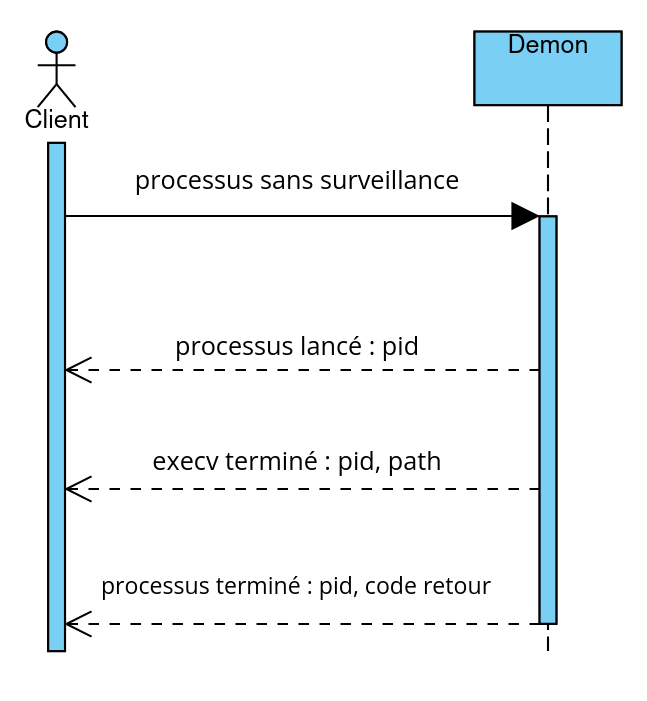
\includegraphics[scale=0.35]{fonctionnement_normal.png}}

\subsubsection{Détail, utilisation de epoll dans le daemon C}

Un détail qui mérite une explication un peu plus poussé est l'utilisation de epoll dans le daemon C. Epoll en c permet de faire comme poll c'est à dire gérer plusieurs file descriptor en même temps mais avec plusieurs fonctionnalité supplémentaire. Celle qui s'est avéré très utile est le fait de pouvoir attacher une structure de données personnalisé à n'importe quel évènement epoll ajouté. Par exemple comme ceci : 

\begin{verbatim}
struct epoll_event ev;
event_data_sock *edata = malloc(sizeof(event_data_sock));
if(edata==NULL){
    free(edata);
    perror("malloc");
    return -1;
}
edata->fd = server_socket->sockfd;
edata->type = SOCK_CONNEXION;
edata->sock_info=server_socket;
ev.events=EPOLLIN;
ev.data.ptr=edata;
if (epoll_ctl(epollfd, EPOLL_CTL_ADD, server_socket->sockfd, &ev)==-1){
    printf("error while trying to add file descriptor to epoll interest list");
    free(edata);
    return -1;
}
\end{verbatim}

L'interet principal est de savoir à quel type de notification on a affaire. Car on ne traite pas une notification de message sur un socket de la même manière qu'une notification provoqué par un signalfd. Mais aussi cela permet de stocker des info supplémentaire nécessaire pour certaine fonctionnalité. Par exemple on devait pouvoir déclancher une notification quand un fichier atteint une certaine taille. Or, inotify ne propose pas nativement cette feature. Alors ce qu'on fait c'est qu'on créer un nouveau file descriptor de type inotify, on y ajoute le fichier, on ajoute les flags comme \texttt{IN\_MODIFY}, puis quand on l'ajoute à epoll on utilise une structure de données personnalisé dans laquelle on stock la taille qui trigger la notification vers le client. Cette méthode a été utilisé de multiple fois, par exemple pour savoir quel fils vient d'exécuter execve ou pour conserver les info du socket servant de serveur pour accepter les connexions arrivantes.

\subsubsection{Implémentation de la sérialisation}

Pour implémenter la sérialisation nous avons commencé par établir un schéma, qui nfous permet de définir des structures de données que l'on va sérialiser.
Nous avons décidé de catégoriser chaque type de message que le client peut envoyer au démon ainsi que ceux que le démon peut envoyer au client comme des \textit{events}. Chaque message sérialisé contient un \textit{event} parmi tout les \textit{events} possibles. Tous les \textit{events} sont nommés et répertoriés dans une \textit{table}, et chaque \textit{event} est ensuite défini plus haut dans le schéma.

\begin{verbatim}
    union Event {
    RunCommand,
    KillProcess,
    EstablishTCPConnection,
    EstablishUnixConnection,

    ExecveTerminated,
    ProcessLaunched,
    ChildCreationError,
    ProcessTerminated,
    TCPSocketListening,
    InotifyPathUpdated,
    InotifyWatchListUpdated,
    SocketWatched,
    SocketWatchTerminated
}

table Message {
    events: Event;
}
\end{verbatim}

\noindent Exemple de la définition d'un \textit{event} : 

\begin{verbatim}
    table ExecveTerminated {
    pid: int32;
    command_name: string;
    success: bool;
}
\end{verbatim}

Nous avons ensuite codé une fonction pour sérialiser et une fonction pour désérialiser chacune des \textit{table} répertoriées dans l'\textit{union} Event. Ce travail a été effectué en Rust pour le démon codé en Rust, en C++ pour le démon codé en C ainsi qu'en Python pour effectuer différents tests sur le démon. 

Nous avons choisi de coder la sérialisation du démon C en C++ car si nous avions travaillé en C, il aurait fallu utiliser un projet à part, FlatCC, qui contient son propre compilateur de schéma ainsi que sa propre bibliothèque en C. Cette solution n'était pas viable car FlatCC n'est pas maintenu de la même manière que Flatbuffers, et la bibliothèque C n'est pas nécessairement mise à jour au même rythme que dans les autres langages, ce qui aurait posé problème. Nous avons préféré rester sur la même dépendance pour tout le projet.

\subsection{Analyse des Performances}

À ce stade, nous avons entièrement intégré le démon dans un système. Nous avons veillé à ce que toutes les fonctionnalités majeures soient couvertes par les tests de régression.\\

Pour comprendre l’efficacité du démon, nous avons conçu et mis en œuvre des outils automatisés de test de performance. Ces outils simulaient des scénarios d’utilisation réels et mesuraient les ressources système consommées par le démon sous différentes charges.\\

Nous avons ensuite recueilli des données de performance telles que la latence, l’utilisation du processeur, et mené une analyse détaillée des résultats (cf. \ref{sec:analyse}). Cela nous a aidés à comprendre les compromis entre l'utilisation de Rust et de C en termes d’efficacité à l'exécution et à choisir l’un des deux.

\subsubsection{Détails}

Grâce au framework de tests, \texttt{pytest} nous avons pu créer des fixtures permettant de réutiliser le code dans plusieurs fonctions de tests. Par exemple pour lancer le démon une fixture s'impose pour pas réécrire le code plusieurs fois.\\

Prototype de tests en pseudo-code : 

\begin{verbatim}
    fn test_sleep(daemon) {
        connect(port)
        send(serialize_command("sleep 3"))
        wait_received_process_launched()
        start_timer()
        wait_received_process_terminated()
        stop_timer()
        assert timer +- 100 == 3
    }
\end{verbatim}

Dans ce test le paramètre \texttt{daemon} est une \textbf{fixture} de notre jeu de tests, il lancera automatiquement le démon sur un \texttt{port} précisé en amont. Ici, on vérifie si une attente de 3 secondes a été détectée avec une marge d’erreur de $\varepsilon$ \textbf{seconde(s)} (100 dans ce cas).

%----------------------------------------------------------------------------------------------

\section{Gestion du projet}


\subsection{Partage des tâches}

La répartition des tâches s'est faite de façon assez naturelle. Mohamed s'est concentré sur la partie sérialisation en Rust et les tests d'overheads. Alexandre s'est occupé de la sérialisation C et python pour permettre la création des tests de régression. Quant à Telmo et Hadrien, ils se sont respectivement occupé de la conception du daemon C et Rust. Enfin les tests de régression ont aussi été conçu par Telmo et Hadrien.  

%----------------------------------------------------------------------------------------------

\section{Analyse}
\label{sec:analyse}
Pour mesurer les performances de nos \texttt{daemons} nous comparons l'overhead généré par rapport à l'appel système d'une commande simple : \textbf{echo}.
Nous mesurons d'abord 20 fois le temps moyen mis par l'appel consécutif de 30 fois \textbf{echo}. Ensuite, au début de chaque test d'un \texttt{daemon}, celui-ci est créé avant de devoir recevoir 30 appels consécutifs de la même commande \textbf{echo}. Là encore nous effectuons une moyenne sur 20 mesures. :


\centerline{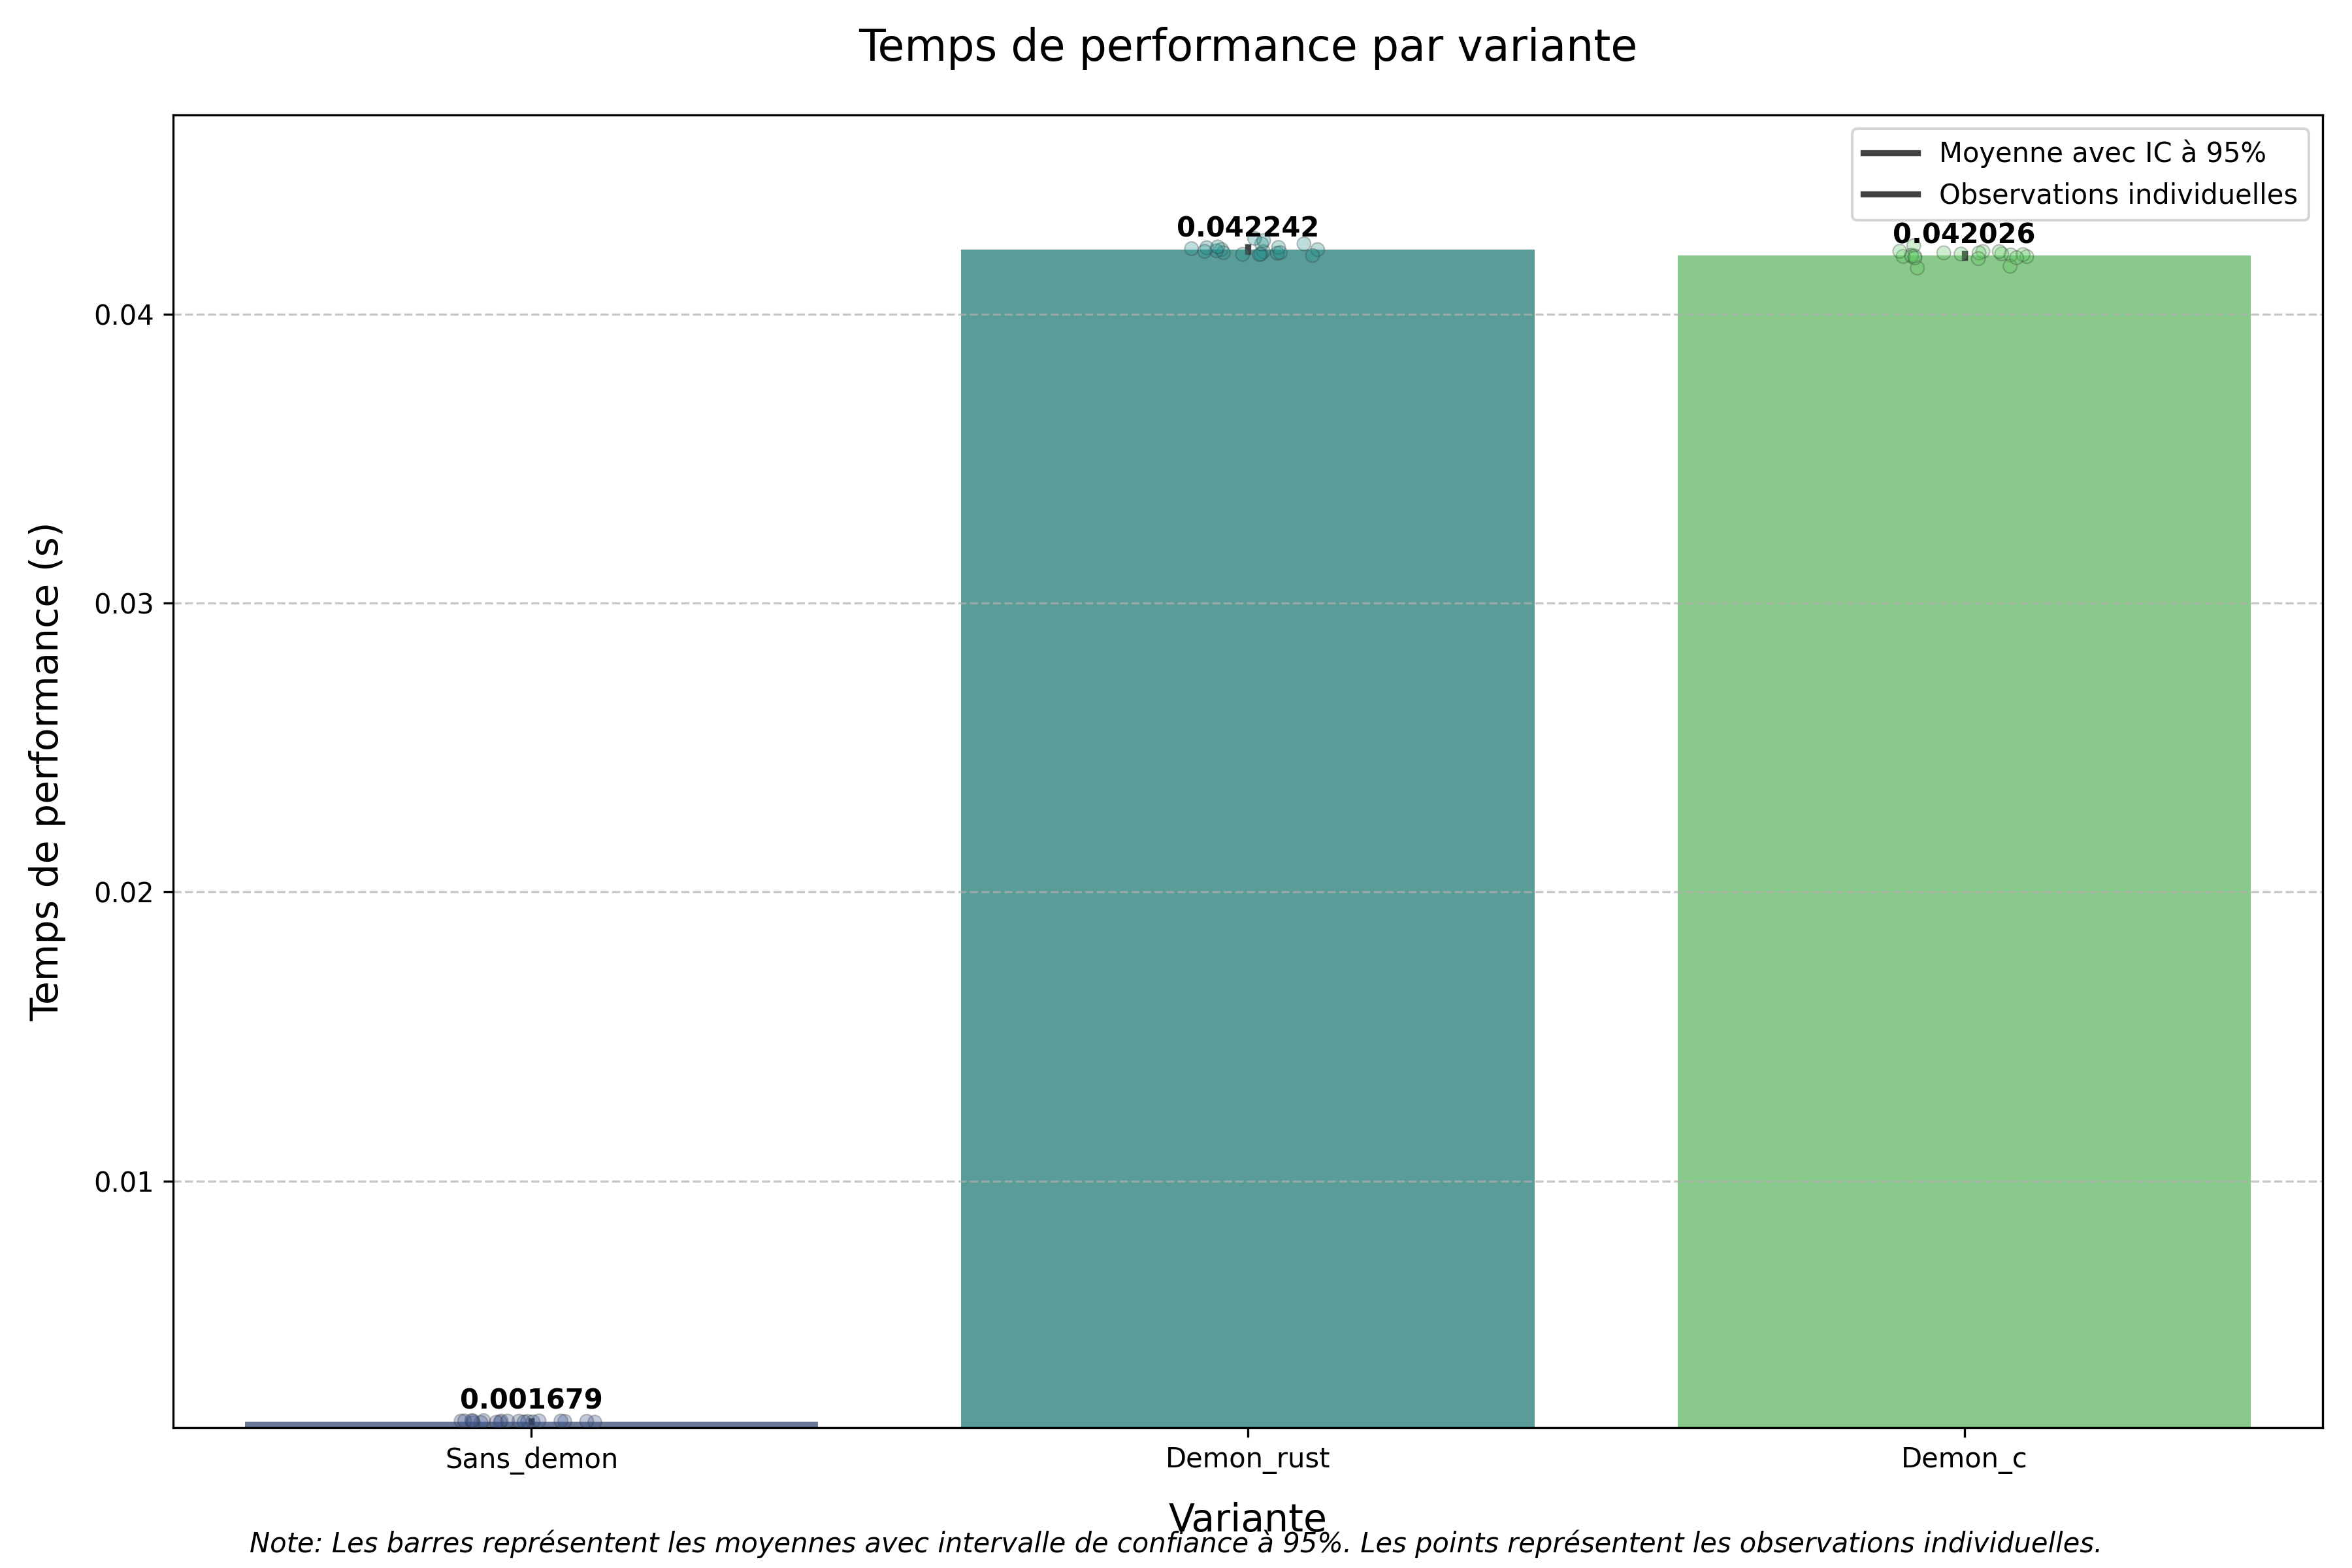
\includegraphics[scale=0.4]{performance_comparison}}

L'appel système d'\textbf{echo} dure en moyenne 0.8 ms, tandis que les \texttt{daemons} en Rust et en C mettent respectivement 42.2 ms et 42.0 ms pour exécuter la commande. L'écart entre ces deux derniers est trop faible pour désigner un \texttt{daemon} plus performant que l'autre sur l'échelle temporelle, si une personne souhaite poursuivre le dévellopement d'un démon elle devra choisir celui avec le language dont elle a le plus d'affinité, ou bien effectuer des mesures sur la consommation de mémoire. De façon plus globale, les \texttt{daemons} lancent l'exécution d'une commande rapidement, l'objectif souhaité de ce projet est donc satisfait. 

%----------------------------------------------------------------------------------------------
\section{Conclusion}

En conclusion, nous avons réussi à produire 2 daemon de contrôle offrant les même fonctionnalités, avec un overhead léger. Le tout avec un layer de sérialisation permettant une communication interlanguage garantissant une certaine flexibilité du coté de l'utilisateur. Cependant, il reste des pistes d'amélioration possible. Par exemple, pour le moment on ne peut avoir qu'un seul client connecté par daemon. La detection de socket se fait de façon synchrone ce qui pourrait être améliorer. On pourrait aussi étendre le schéma Flatbuffers pour, par exemple, proposer plus de type d'évènement différent au moment de la reception d'une notification inotification inotify. On pourrait aussi permettre à l'utilisateur de décider du timeout pour la detection de socket. On pourrait ajouter la possibilité de créer et détecter des socket unix. Enfin à l'heure actuel, il n'est aussi pas possible de supprimer, depuis le coté client, un évènement inotify déjà ajouté.
Bref, le code fourni n'est qu'une base sur laquelle étendre les fonctionnalités au grés des besoins.  


\end{document}
